%%%
%%% V10
%%%

	Alte Sprachen, die auch heute noch in Verwendung sind, sind vor allem \textbf{Lisp} und
	\textbf{COBOL}. Neuere Sprachen, wie bspw. \textbf{Swift}, haben Züge von Lisp.
	\begin{flalign*}
		 \left.\begin{array}{c}
		 	\text{Emacs}\\
		 	\text{AutoCAD}\\
		 	\text{InterleatTPS}\\
		 	\text{R}
		 \end{array}\right\}\text{ bauen auf Lisp auf}
	\end{flalign*}

	%%% snippet V11

	\subsection{Eigenschaften von Lips} % (fold)
	\label{sub:eigenschaften_von_lips}
	
	\begin{itemize}
		\item stateful
		\item dynamic typing
		\item program as data
		\item s-expressions, z.B. \texttt{(+ 3 4 5)}\\
		\begin{tikzpicture}
			\node {\texttt{+}}
				child { node {\texttt{3}}}
				child { node {\texttt{4}}}
				child { node {\texttt{5}}};
		\end{tikzpicture}
	\end{itemize}

	% subsection eigenschaften_von_lips (end)

	%%% snippet V11

	\lstLisp[Auswertung des Ausdrucks durch \texttt{'} verhindern]
	\begin{lstlisting}
(quote (1 2 3)) = '(1 2 3)
	\end{lstlisting}

	\subsection{Listen-Konzept} % (fold)
	\label{sub:listen_konzept}
	
		Lisp-Programme sind Listen von Symbolen und Ausdrücken.

		\lstLisp[Liste in Lisp]
		\begin{lstlisting}
(1 2)
		\end{lstlisting}

		\lstHaskell[Liste in Haskell]
		\begin{lstlisting}
[1,2] == 1:2:[]
		\end{lstlisting}

		\begin{figure}[H]
			\centering
			\caption{Veranschaulichung des vorherigen Listenbeispieles}
			\vspace*{-15pt}
			\rotatebox{-90}{
				\tikzstyle{cell} = [draw,ellipse,ellipse split]
				\tikzstyle{leaf} = [draw,circle]
				\begin{tikzpicture}
				  \node (1) at (0,0)  [cell]{};
				  \node (2) at (1,-1) [leaf]{\rotatebox{90}{1}};
				  \node (3) at (1,1)  [cell]{};
				  \node (4) at (2,0)  [leaf]{\rotatebox{90}{2}};
				  \node (5) at (2,2)  {};
				  \path (1) edge [->,thick,out=-45,in=180] (2);
				  \path (1) edge [->,thick,out=45,in=180] (3);
				  \path (3) edge [->,thick,out=-45,in=180] (4);
				  \path (3) edge [-|,thick,out=45,in=180] (5);
				\end{tikzpicture}
			}
		\end{figure}
		\begin{figure}[H]
			\centering
			\caption{Veranschaulichung Listenelement allgemein}
			\vspace*{-15pt}
			\rotatebox{-90}{
				\tikzstyle{cell} = [draw,ellipse,ellipse split]
				\begin{tikzpicture}
				  \node (1) at (0,0)  [cell]{};
				  \node (2) at (-1,-1) {\rotatebox{90}{car}};
				  \node (3) at (-1,1)  {\rotatebox{90}{cdr}};
				  \path (1) edge [thick,out=225,in=0] (2);
				  \path (1) edge [thick,out=135,in=0] (3);
				\end{tikzpicture}
			}
		\end{figure}
		\begin{figure}[H]
			\centering
			\caption{1-elementige Liste \texttt{(1)}}
			\vspace*{-15pt}
			\rotatebox{-90}{
				\tikzstyle{cell} = [draw,ellipse,ellipse split]
				\tikzstyle{leaf} = [draw,circle]
				\begin{tikzpicture}
				  \node (1) at (0,0)  [cell]{};
				  \node (2) at (1,-1) [leaf]{\rotatebox{90}{1}};
				  \node (3) at (1,1)  {};
				  \path (1) edge [->,thick,out=-45,in=180] (2);
				  \path (1) edge [->,thick,out=45,in=180] (3);
				\end{tikzpicture}
			}
		\end{figure}
		
		\begin{figure}[H]
			\centering
			\caption{Selbstreferenzen sind möglich}
			\vspace*{-40pt}
			\rotatebox{-90}{
				\tikzstyle{cell} = [draw,ellipse,ellipse split]
				\tikzstyle{leaf} = [draw,circle]
				\begin{tikzpicture}
				  \node (1) at (0,0)  [cell]{};
				  \node (2) at (1,-1) [leaf]{\rotatebox{90}{1}};
				  \path (1) edge [->,thick,out=-45,in=180] (2);
				  \draw (1) edge [->,thick,out=45,in=180,looseness=8] (1);
				\end{tikzpicture}
			}
		\end{figure}
		
		\begin{figure}[H]
			\centering
			\caption{\texttt{'\#1=(\#1\# . \#1\#)}}
			\vspace*{-35pt}
			\rotatebox{-90}{
				\tikzstyle{cell} = [draw,ellipse,ellipse split]
				\begin{tikzpicture}
				  \node (1) at (0,0)  [cell]{};
				  \draw (1) edge [->,thick,out=-45,in=180,looseness=8] (1);
				  \draw (1) edge [->,thick,out=45,in=180,looseness=8] (1);
				\end{tikzpicture}
			}
		\end{figure}
		
		\begin{figure}[H]
			\centering
			\caption{\texttt{'\#1=(1 2 3 . \#1\#)}}
			\vspace*{-70pt}
			\rotatebox{-90}{
				\tikzstyle{cell} = [draw,ellipse,ellipse split]
				\tikzstyle{leaf} = [draw,circle]
				\begin{tikzpicture}
				  \node (1) at (0,0)  [cell]{};
				  \node (2) at (1,-1) [leaf]{\rotatebox{90}{1}};
				  \node (3) at (1,1)  [cell]{};
				  \node (4) at (2,0) [leaf]{\rotatebox{90}{2}};
				  \node (5) at (2,2)  [cell]{};
				  \node (6) at (3,1) [leaf]{\rotatebox{90}{3}};
				  \path (1) edge [->,thick,out=-45,in=180] (2);
				  \path (1) edge [->,thick,out=45,in=180] (3);
				  \path (1) edge [->,thick,out=-45,in=180] (2);
				  \path (1) edge [->,thick,out=45,in=180] (3);
				  \path (3) edge [->,thick,out=-45,in=180] (4);
				  \path (3) edge [->,thick,out=45,in=180] (5);
				  \path (5) edge [->,thick,out=-45,in=180] (6);
				  \path (5) edge [->,thick,out=45,in=180,looseness=2] (1);
				\end{tikzpicture}
			}
		\end{figure}

	% subsection listen_konzept (end)

	\subsection{Closures} % (fold)
	\label{sub:closures}
	
	Umsetzung in Haskell

	\lstHaskell
	\begin{lstlisting}
obj = let x = 1
      in \() -> x <- x+1
	\end{lstlisting}

%%%
%%% end V10
%%%

%%%
%%% V11
%%%

		oder auch

		\lstHaskell
		\begin{lstlisting}
f = let a = 7 in \() -> a
		\end{lstlisting}

		ein Aufruf zeigt dann Folgendes

		\lstHaskell
		\begin{lstlisting}
f()
> 7
		\end{lstlisting}

		\begin{figure}[hb]
			\caption{Aufbau einer Haskell-Closure}
			
\includegraphics[width=\textwidth]{workfiles/v11_1}
		\end{figure}
		Hier liegt \texttt{var} liegt ausserhalb der Funktion \texttt{\textbackslash() -> a}. Die \texttt{var} müssen gültig sein.

		\lstHaskell[\texttt{let} in Haskell]
		\begin{lstlisting}
let a = 2
    b = 7
    ...
in ...
		\end{lstlisting}

		\lstLisp[\texttt{let} in Lisp]
		\begin{lstlisting}
(let ((v1 exp) (v2 exp)) e1 e2 ... en)
		\end{lstlisting}

		Bei obigem Beispiel ist en die Ausgabe bzw. das Ergebnis des Gesamtausdrucks.\\

		Variableneigenschaften in Lisp, Anm.: Hier fehlen die Live-Demos aus der Vorlesung.\\

		\begin{tabular}{rlll}
			& \textbf{Scope}	& \textbf{Extent} &  \\
		a	& lexical		& indefinite	& closures \\
		b	& indefinite	& dynamic		& special \\
		\end{tabular}$\;$\\

		Variablen festlegen in verschiedenen Sprachen:
		\begin{verbatim}
a := 150     Pascal
a = 150;     C
(setq a 150) Lisp
		\end{verbatim}

		\lstLisp[Spezialvariablen]
		\begin{lstlisting}
(declaim (special b))
		\end{lstlisting}

		Solche Spezialvariablen haben einen Stack von Werten, auf den beim Betreten von Scopes die Werte abgelegt werden.

		\lstHaskell[Anonyme Funktion]
	\begin{lstlisting}
\x -> x + x
		\end{lstlisting}

		\lstLisp[Anonyme Funktion]
		\begin{lstlisting}
(lambda (x) (+ x x))
		\end{lstlisting}

		\begin{figure}[H]
			\caption{Objekt-Aufbau in der ooP}
			
\includegraphics[width=\textwidth]{workfiles/v11_2}
		\end{figure}

		\begin{figure}[H]
			\centering
			\caption{Doppelbelegung von \texttt{max} (Live-Demo)}
			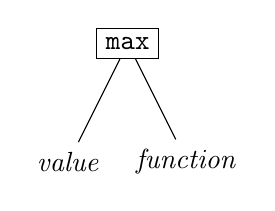
\begin{tikzpicture}
				\node [draw, rectangle] {\texttt{max}}
					child { node {\emph{value}}}
					child { node {\emph{function}}};
			\end{tikzpicture}
		\end{figure}

		Closures sind Grundlage für die ooP.

		\begin{figure}[H]
			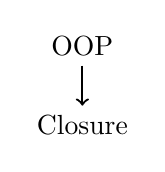
\begin{tikzpicture}
				\node (1) at (0,0) {OOP};
				\node (2) at (0,-1) {Closure};
				\path (1) edge [->,thick] (2);
			\end{tikzpicture}
		\end{figure}

	% subsection closures (end)

%%%
%%% end V11
%%%